\chapter{Algorithms}\label{chap:Algorithms}
% =============================================================================
\section{Scholar Plot Design - Base Level}
% =============================================================================
The base level of Scholar Plot (SP) visualizes individual academic records. The first issue we had to address as part of the design process for this level was to determine what to visualize. To answer this question we looked at the merit criteria considered by promotion, tenure, and search committees; these are: a) publication quality and quantity, and b) research funding. Furthermore, publication quality is defined by two factors: citation counts and prestige of the journals where the publications appeared. 

Accordingly, we decided to structure individual scholar plots as two-panel arrangements - the top panel visualizing the individual's publication record, while the bottom panel visualizing the individual's research funding record (Fig. \ref{fig:ScholarPlot}). This arrangement brings to the fore any causal relationship that may exist between funding and publishing, as publication production is often powered by research dollars. The common timeline in the horizontal axes of the two panel graphs facilitates such an association. 

\begin{figure*}
%  \begin{minipage}{\columnwidth}
    \centering
    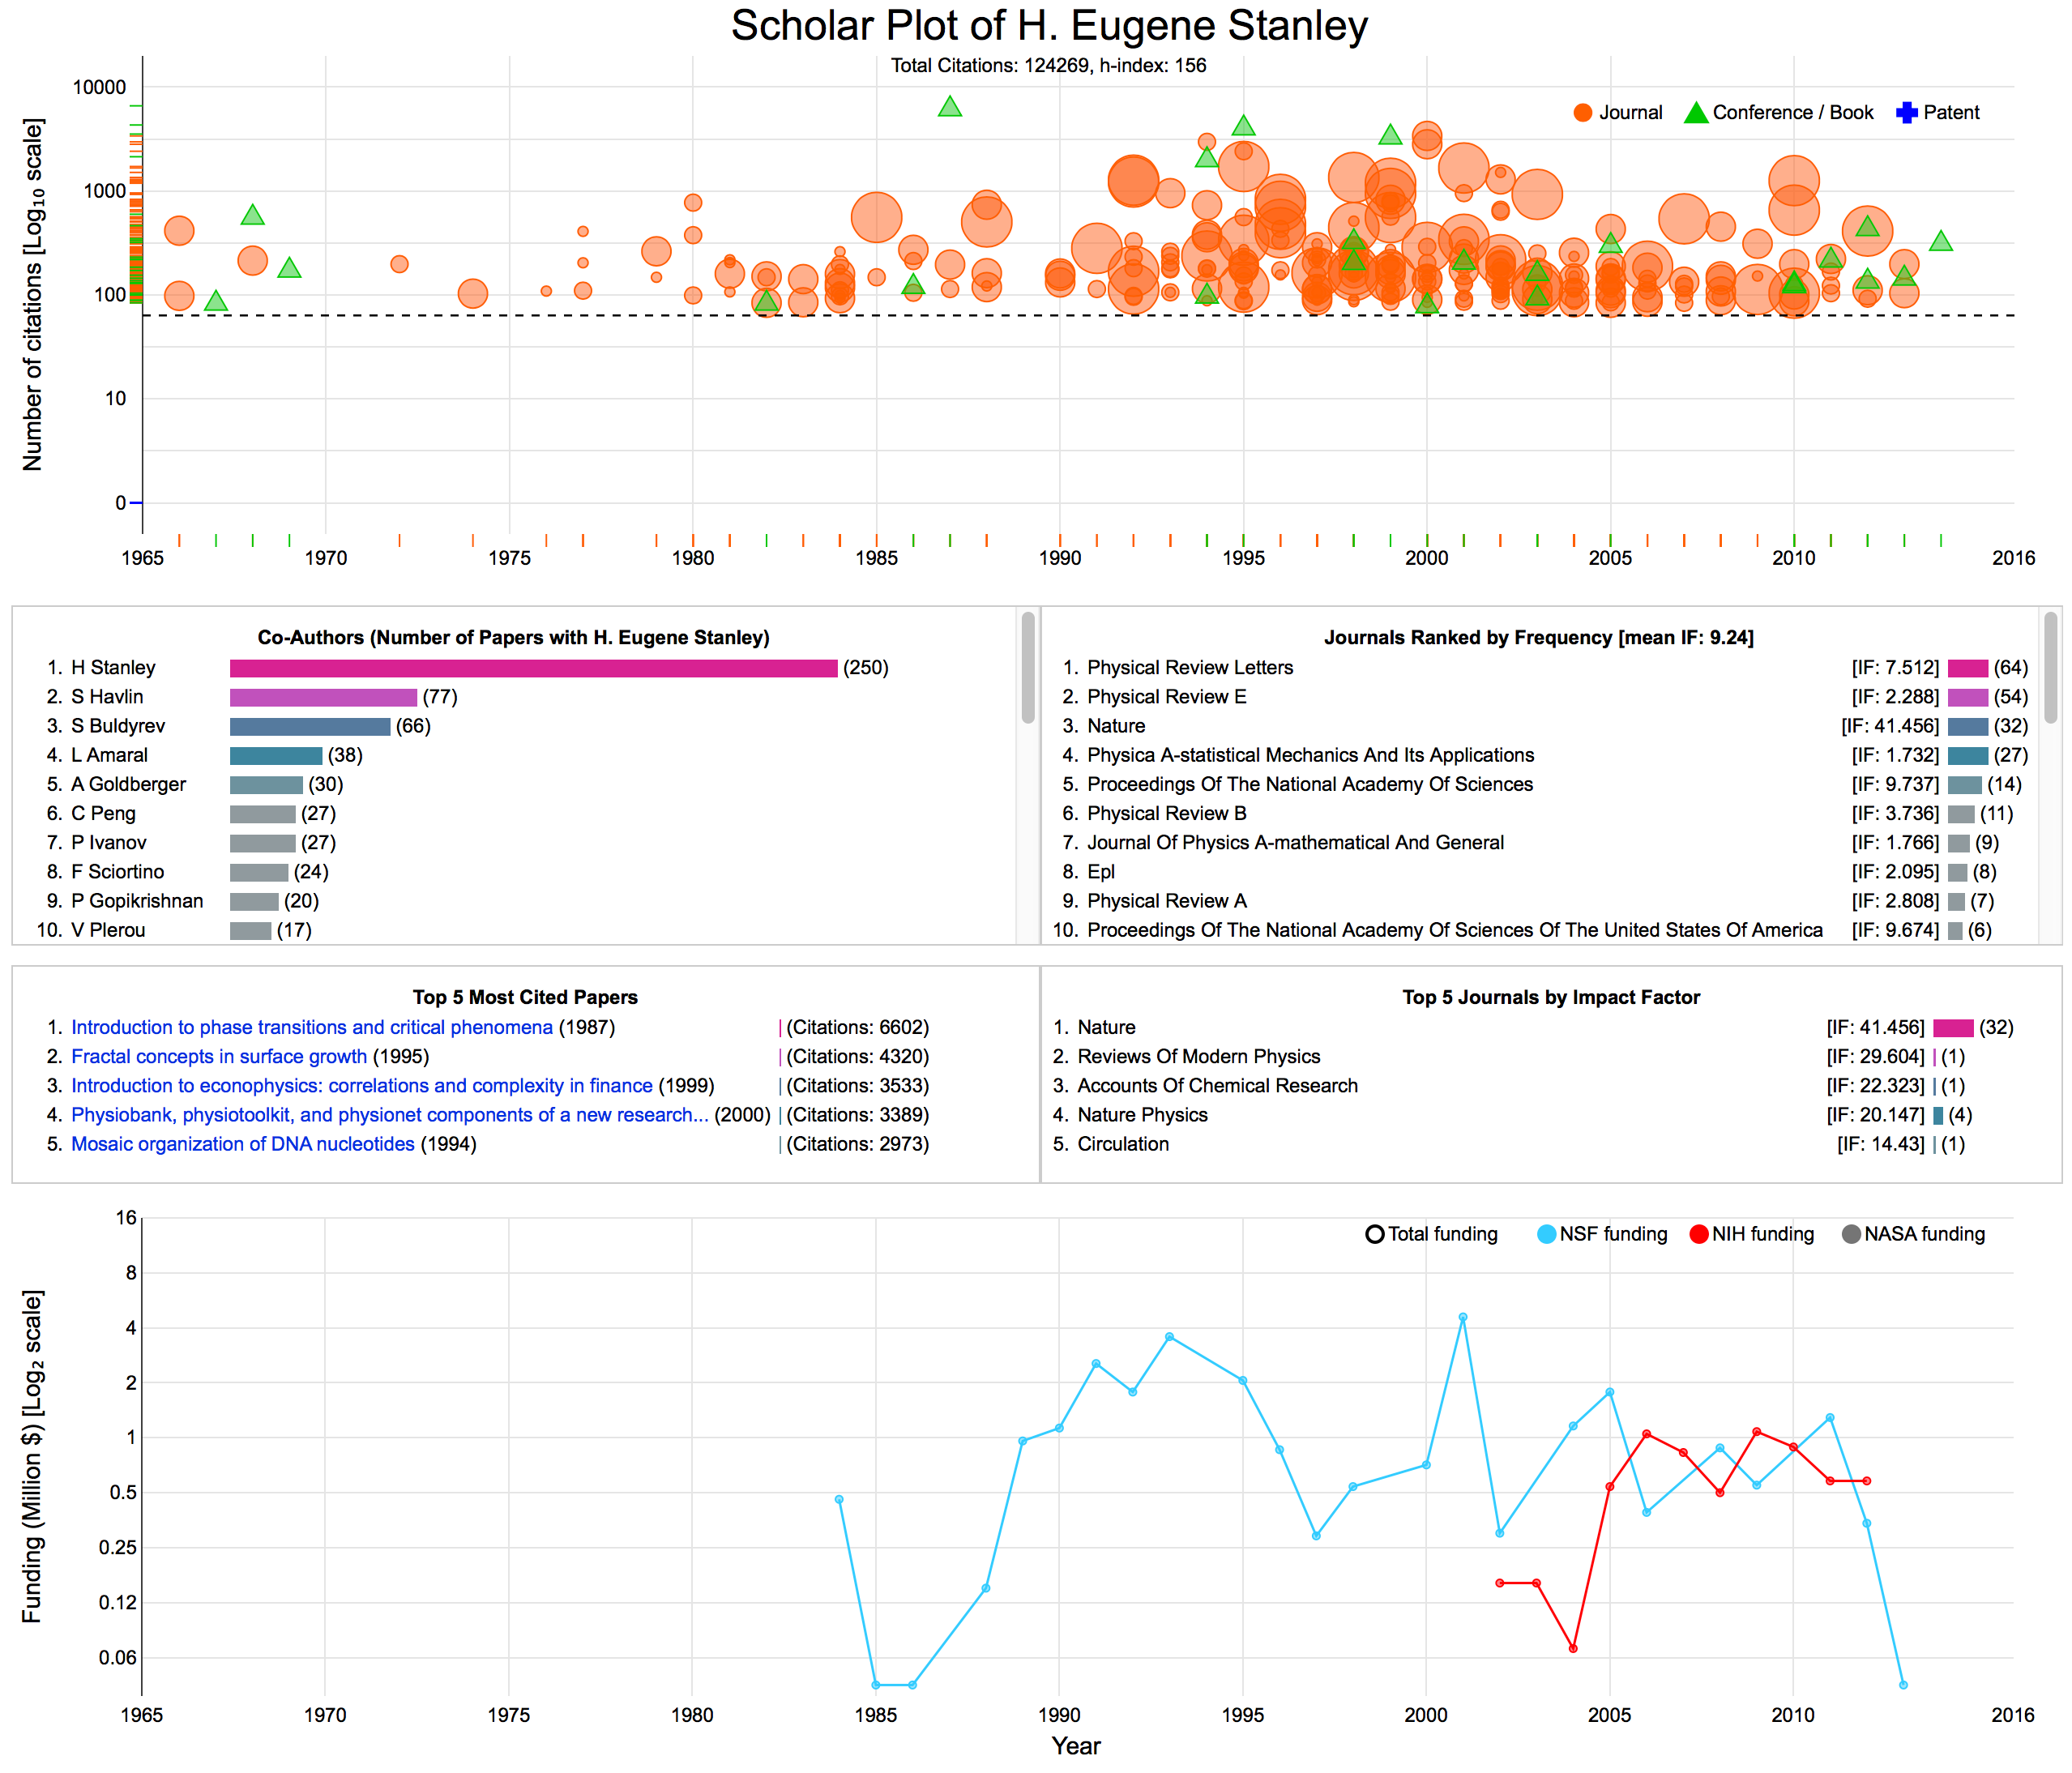
\includegraphics[width=0.8\textwidth]{figures/fig-EugeneStanley}
    \caption{Base level Scholar Plot (SP) example - a famous physicist and interdisciplinary scientist with dozen of articles in \emph{Nature}. The summary panels in the middle were added after feedback from the focus group. Notice how this scholar's publication production exploded in sync with the commencement of substantial federal funding.}~\label{fig:ScholarPlot} 
%    \end{minipage}
\end{figure*} 

The vertical axis of the publication graph indexes citation counts (Fig. \ref{fig:ScholarPlot}) - an important quality indicator for a publication. As we mentioned, the prestige of the publication venue is another important quality indicator. We convey this additional measurement dimension by varying the size of the graph points. 

Only journals have a widely accepted ranking system reflecting prestige - the Journal Impact Factor (IF) List, issued every year by Thomson Reuters. Hence, we opted to represent different publication types with different symbols,  varying the symbol size of  journal publications only, for which an established ranking system exists. We chose disks to be the symbols of journal publications, as disk scaling can be done very effectively by simply varying its radius ($A \sim r^2$). Specifically, after performing histogram analysis on the IFs of journal publications, we settled on four disk sizes to represent journal prestige: $\#1 < \#2 < \#3 < \#4$ (Fig. \ref{fig:symbols}). We found that the great majority of journal publications appear in journals with $\mbox{IF} < 2$, assigning to this cohort the smallest disk size symbol, $\# 1$.  These are mid-level specialized technical and scientific journals. The next IF bracket  ($2 \leq \mbox{IF} < 4$) includes high quality specialized technical (e.g., IEEE Transactions) and scientific journals represented by disk \#2. The third IF bracket ($4 \leq \mbox{IF} < 16$) includes  very high quality science journals and specialized medical journals represented by disk  \#3. The top IF bracket ($\mbox{IF} \geq 16$) includes famous general science journals (e.g., \emph{Nature}) and top medical journals (e.g., \emph{New England Journal of Medicine}); they are assigned the largest disk, $\#4$.

In the funding graph, each funding agency is represented by a polyline with a characteristic color (Fig. \ref{fig:ScholarPlot}). Grants are reported at the year they were awarded. If more than one grant was awarded by the same agency the same year to the specific investigator, then the full list shows up by rolling the mouse over the corresponding point in the polyline.

The end effect of this simple visualization scheme is a picture that does not only compress dozens of CV pages, but also brings to the fore nuanced information about an academic's profile that can be grasped at a glance. Here are some examples:
\begin{figure*}
%  \begin{minipage}{\columnwidth}
    \centering
    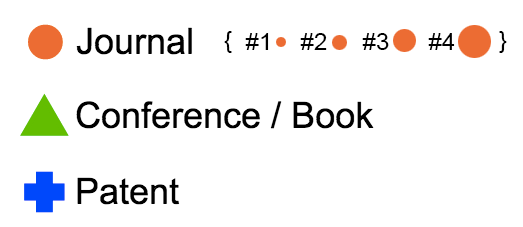
\includegraphics[width=0.8\textwidth]{figures/fig-disksize}
    \caption{Publication symbols.}
    \label{fig:symbols} 
%    \end{minipage}
\end{figure*}
\begin{enumerate}
\item It is easy to identify what type of publication powers the individual's scholarship - a correlate of disciplinary culture. For example, it is easy to spot career profiles of computer scientists and engineers (Fig. \ref{fig:Splots}a), where typically scholarship is built on conference rather than journal publications.
\item It is easy to identify if the individual's scholarship is heavily associated with high or mid/low IF journals. If the publication graph is full of mid or small disks, this indicates that the scholar has done prolific methodological work that appeared in good specialized journals (Fig. \ref{fig:Splots}b). If the publication graph is full of large disks, this indicates that the scholar has done trendy and novel work that appeared in famous journals (Fig. \ref{fig:Splots}c).
\item It is easy to identify if high funding levels yield high quantity and quality of publications or not (Fig. \ref{fig:ScholarPlot}). This may be especially useful to NSF and NIH reviewers who assess among other things the quality and impact of the investigator's prior work for the funding amounts s/he received.
\begin{figure*}
    \centering
    \subfigure[SP of an accomplished Engineer.]{%
    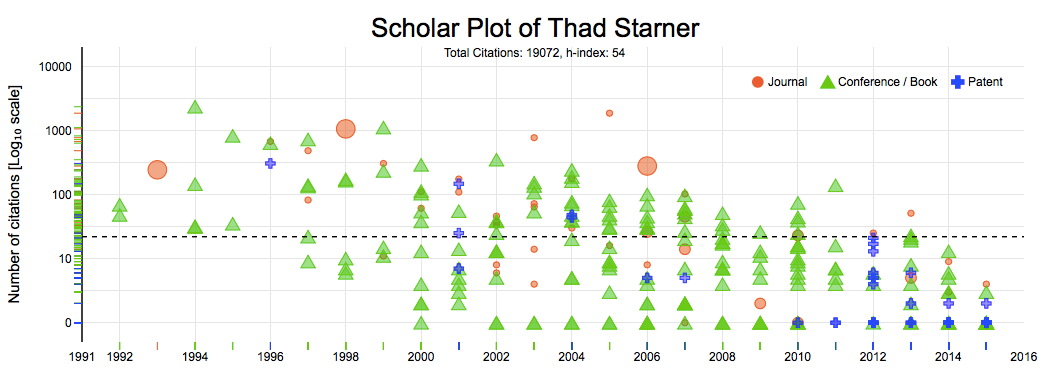
\includegraphics[width=1.0\marginparwidth]{figures/fig-ThadStarner}
    } \\
    \subfigure[SP of an accomplished Physicist.]{%
     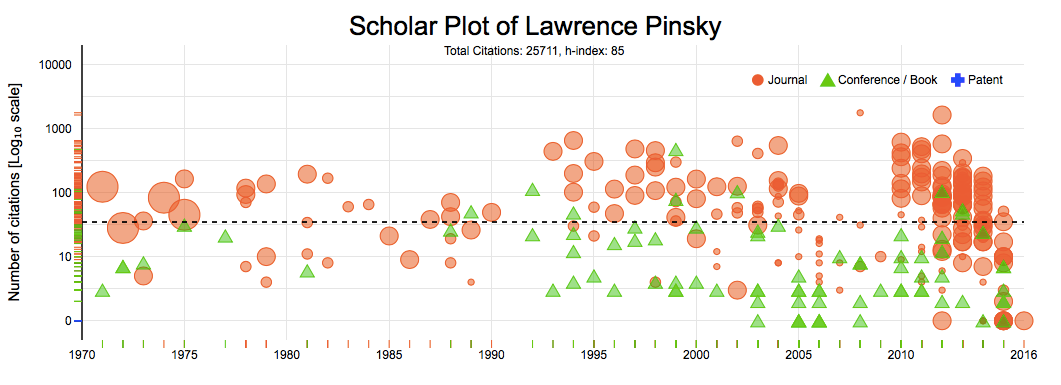
\includegraphics[width=1.0\marginparwidth]{figures/fig-LawrencePinsky}
     }\\
      \subfigure[SP of a famous Interdisciplinarian.]{%
     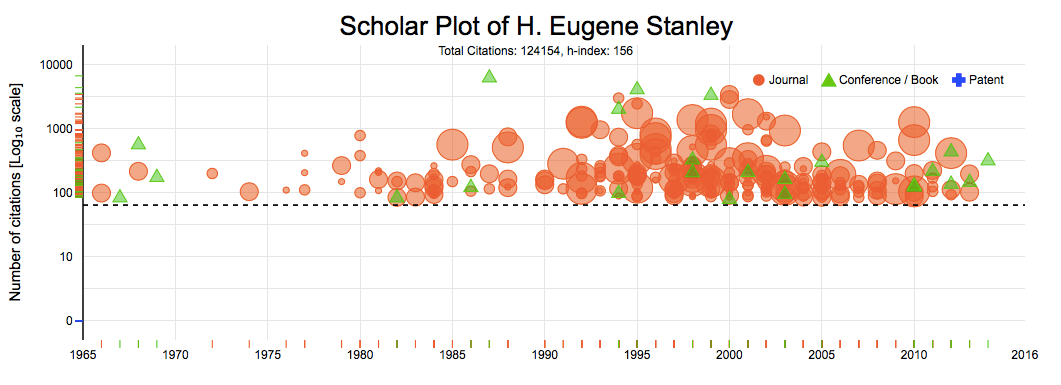
\includegraphics[width=1.0\marginparwidth]{figures/fig-EugeneStanley-pub}
     }
     \caption{}~\label{fig:Splots} 
\end{figure*} 
\end{enumerate}

% =============================================================================
\section{Scholar Plot Data Sources}
% =============================================================================
There were several options to get bibliographic data for powering the publication graph of Scholar Plot (SP). These included \href{http://www.scopus.com/}{Scopus}, \href{http://www.isiknowledge.com/}{ISI Web of Knowledge}, and \href{http://scholar.google.com}{Google Scholar}. We chose Google Scholar for two reasons: a) it is all inclusive, covering all types of publications, that is, journals, conferences, books, and patents; and, b) it is freely available.

Our choice carries a few challenges, too. Google Scholar does not provide an application programming interface. Hence, we had to develop elaborate software to scrape information off publicly available Google Scholar pages. Also, not every academic has a Google Scholar page. This has been changing fast, however, as one college after the other in the United States mandating their faculty to maintain a Google Scholar page. 

We use the Journal IF List issued every year by Thompson Reuters to assign disk sizes to journal publications.

For funding records, we use the publicly available grant records from the \href{http://www.nsf.gov/awardsearch/download.jsp}{National Science Foundation (NSF)}, the \href{http://exporter.nih.gov/ExPORTER_Catalog.aspx}{National Institutes of Health (NIH)}, and the \href{https://www.research.gov/research-portal/appmanager/base/desktop?_nfpb=true&_eventName=viewQuickSearchFormEvent_so_rsr}{National Aeronautics and Space Administration (NASA)}. These are the only funding agencies with publicly available datasets at this point.
